% Copyright (c) 2013 Alexander Bluhm <bluhm@openbsd.org>
%
% Permission to use, copy, modify, and distribute this software for any
% purpose with or without fee is hereby granted, provided that the above
% copyright notice and this permission notice appear in all copies.
%
% THE SOFTWARE IS PROVIDED "AS IS" AND THE AUTHOR DISCLAIMS ALL WARRANTIES
% WITH REGARD TO THIS SOFTWARE INCLUDING ALL IMPLIED WARRANTIES OF
% MERCHANTABILITY AND FITNESS. IN NO EVENT SHALL THE AUTHOR BE LIABLE FOR
% ANY SPECIAL, DIRECT, INDIRECT, OR CONSEQUENTIAL DAMAGES OR ANY DAMAGES
% WHATSOEVER RESULTING FROM LOSS OF USE, DATA OR PROFITS, WHETHER IN AN
% ACTION OF CONTRACT, NEGLIGENCE OR OTHER TORTIOUS ACTION, ARISING OUT OF
% OR IN CONNECTION WITH THE USE OR PERFORMANCE OF THIS SOFTWARE.

\documentclass[14pt]{beamer}
\usetheme{Frankfurt}
\usepackage{tikz}
\author{Alexander Bluhm}
\title{Zero-Copy Socket Splicing}
\institute{OpenBSD and genua}
\date{\today}

\begin{document}

\begin{frame}
\titlepage
\end{frame}

\section{Motivation}

\begin{frame}{Application Level Gateway}
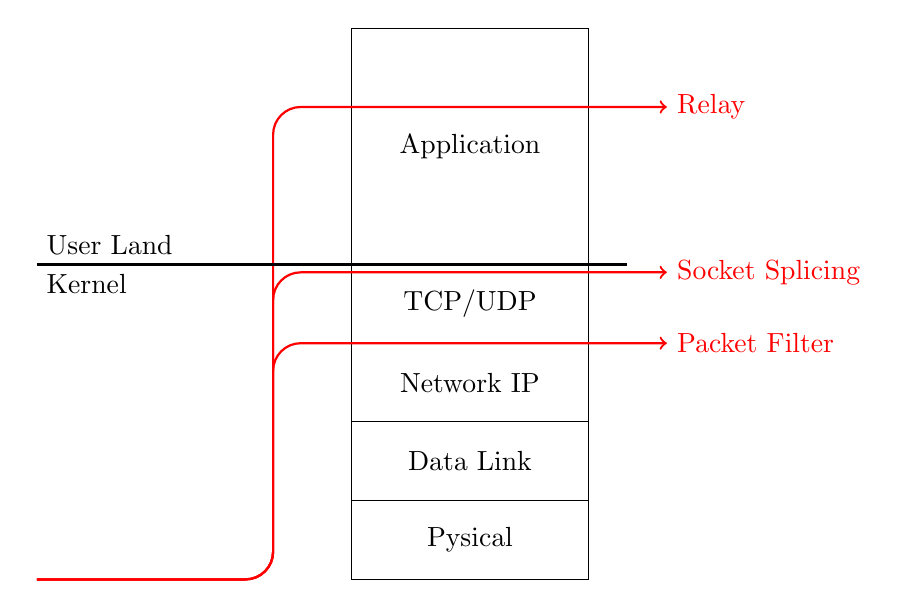
\begin{tikzpicture}
\draw (-1,0) rectangle +(3,1) node(l1) [midway] {Pysical};
\draw (-1,1) rectangle +(3,1) node(l2) [midway] {Data Link};
\draw (-1,2) rectangle +(3,1) node(l3) [midway] {Network IP};
\draw (-1,3) rectangle +(3,1) node(l4) [midway] {TCP/UDP};
\draw (-1,4) rectangle +(3,3) node(l5) [midway] {Application};
\begin{scope}[->,rounded corners=10,thick,red]
\draw (-5,0) -- ++(3,0) -- ++(0,3) -- ++(5,0) node [right] {Packet Filter};
\draw (-5,0) -- ++(3,0) -- ++(0,6) -- ++(5,0) node [right] {Relay};
\end{scope}
\pause
\draw[thick] (-5,4) node(context) {} -- +(7.5,0);
\node [below right] at (context) {Kernel};
\node [above right] at (context) {User Land};
\begin{scope}[->,rounded corners=10,thick,red]
\draw (-5,0) -- ++(3,0) -- ++(0,3.9) -- ++(5,0) node [right] {Socket Splicing};
\end{scope}
\end{tikzpicture}
\end{frame}

\begin{frame}{Persistent HTTP Filtering}
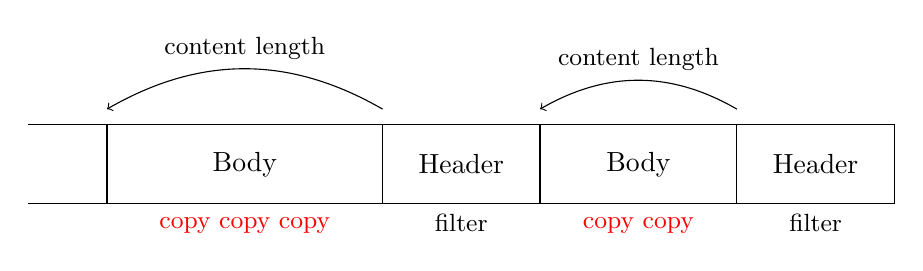
\begin{tikzpicture}
\draw
    (0,0) -- ++(1,0) -- ++(0,1) -- +(-1,0)
    ++(0,-1)  rectangle ++(3.5,1) node (b2) [midway] {Body}
    { [current point is local] ++(0,.2) edge [->,bend right] 
	node [above,font=\small] {content length} ++(-3.5,0) }
    ++(0,-1)  rectangle ++(2,1)   node (h2) [midway] {Header}
    ++(0,-1)  rectangle ++(2.5,1) node (b1) [midway] {Body}
    { [current point is local] ++(0,.2) edge [->,bend right] 
	node [above,font=\small] {content length} ++(-2.5,0) }
    ++(0,-1)  rectangle ++(2,1)   node (h1) [midway] {Header};
\path
    (node cs:name=b2,anchor=south) +(0,-.5) node [font=\small,red]
	{copy copy copy}
    (node cs:name=h2,anchor=south) +(0,-.5) node [font=\small] {filter}
    (node cs:name=b1,anchor=south) +(0,-.5) node [font=\small,red] {copy copy}
    (node cs:name=h1,anchor=south) +(0,-.5) node [font=\small] {filter};
\end{tikzpicture}
\end{frame}

\begin{frame}{HTTP Socket Splicing}
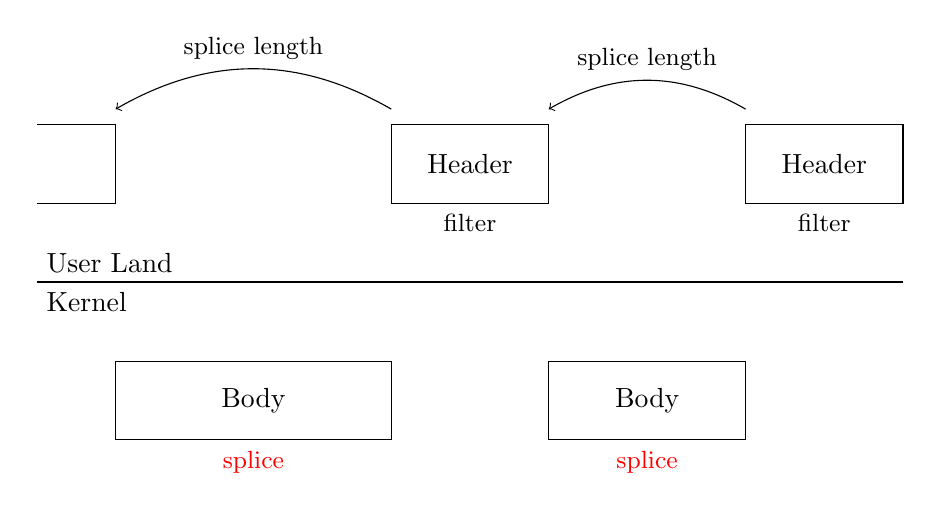
\begin{tikzpicture}
\draw
    (0,+1) -- ++(1,0) -- ++(0,1) -- +(-1,0)
    ++(0,-4)  rectangle ++(3.5,1) node (b2) [midway] {Body}
    { [current point is local] ++(0,3.2) edge [->,bend right] 
	node [above,font=\small] {splice length} ++(-3.5,0) }
    ++(0,+2)  rectangle ++(2,1)   node (h2) [midway] {Header}
    ++(0,-4)  rectangle ++(2.5,1) node (b1) [midway] {Body}
    { [current point is local] ++(0,3.2) edge [->,bend right] 
	node [above,font=\small] {splice length} ++(-2.5,0) }
    ++(0,+2)  rectangle ++(2,1)   node (h1) [midway] {Header};
\path
    (node cs:name=b2,anchor=south) +(0,-.5) node [font=\small,red] {splice}
    (node cs:name=h2,anchor=south) +(0,-.5) node [font=\small] {filter}
    (node cs:name=b1,anchor=south) +(0,-.5) node [font=\small,red] {splice}
    (node cs:name=h1,anchor=south) +(0,-.5) node [font=\small] {filter};
\draw[thick] (0,0) node(context) {} -- +(11,0);
\node [below right] at (context) {Kernel};
\node [above right] at (context) {User Land};
\end{tikzpicture}
\end{frame}

\section{Kernel MBuf}

\begin{frame}{MBuf Data}
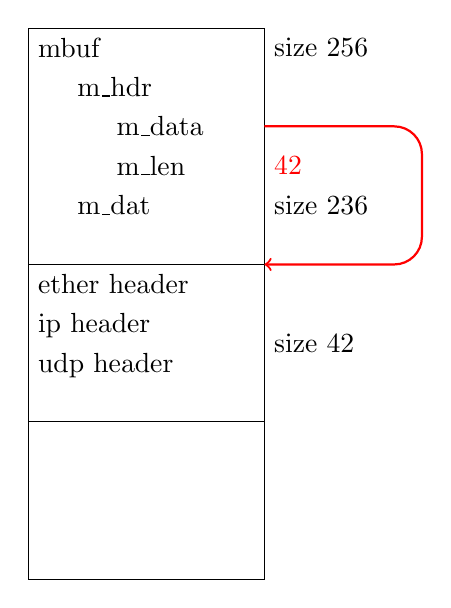
\begin{tikzpicture}
\draw
      ( 0  , 0  ) rectangle +(3,-7)
    ++( 0  , 0  ) node [below right] (mbuf)    {mbuf}
    ++(  .5,- .5) node [below right]           {m\_hdr}
    ++(  .5,- .5) node [below right] (mdata)   {m\_data}
    ++( 0  ,- .5) node [below right] (mlen)    {m\_len}
    ++(- .5,- .5) node [below right] (mdat)    {m\_dat}
      ( 0  ,-3  ) -- +(3,0)
    ++( 0  , 0  ) node [below right] {ether header}
    ++( 0  ,- .5) node [below right] {ip header}
    ++( 0  ,- .5) node [below right] {udp header}
      ( 0  ,-5  ) -- +(3,0);
\path
    (mbuf    -| 3,0) node [right] {size 256}
    (mlen    -| 3,0) node [right,red] {42}
    (mdat    -| 3,0) node [right] {size 236}
      ( 3  ,-4  )    node [right] {size 42};
\draw[->,rounded corners=10,thick,red]
    (mdata   -| 3,0) -| (5,-3) -- (3,-3);
\end{tikzpicture}
\end{frame}

\begin{frame}{MBuf Data Chaining}
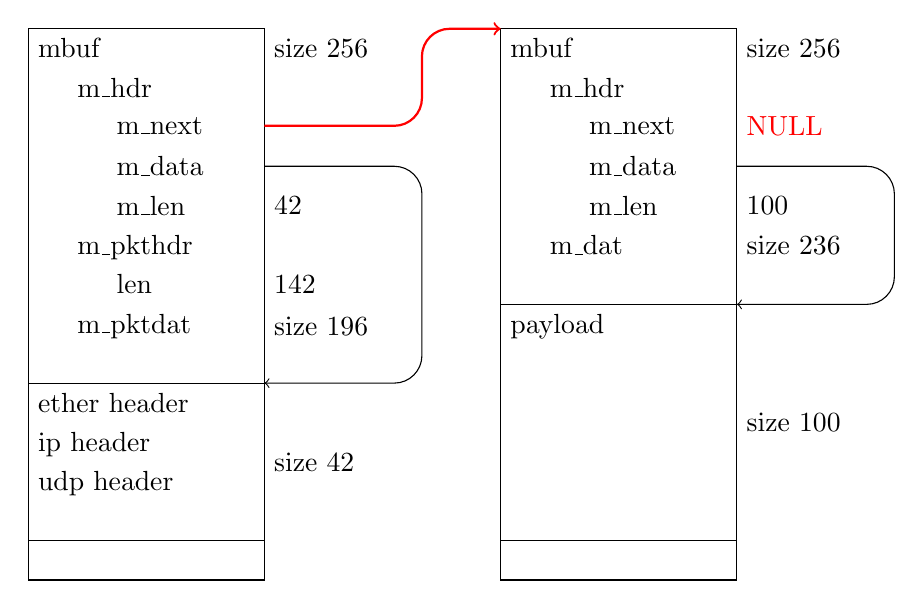
\begin{tikzpicture}
\draw
      ( 0  , 0  ) rectangle +(3,-7)
    ++( 0  , 0  ) node [below right] (mbuf0)    {mbuf}
    ++(  .5,- .5) node [below right]            {m\_hdr}
    ++(  .5,- .5) node [below right] (mnext0)   {m\_next}
    ++( 0  ,- .5) node [below right] (mdata0)   {m\_data}
    ++( 0  ,- .5) node [below right] (mlen0)    {m\_len}
    ++(- .5,- .5) node [below right]            {m\_pkthdr}
    ++(  .5,- .5) node [below right] (len0)     {len}
    ++(- .5,- .5) node [below right] (mpktdat0) {m\_pktdat}
      ( 0  ,-4.5) -- +(3,0)
    ++( 0  , 0  ) node [below right] {ether header}
    ++( 0  ,- .5) node [below right] {ip header}
    ++( 0  ,- .5) node [below right] {udp header}
      ( 0  ,-6.5) -- +(3,0);
\path
    (mbuf0    -| 3,0) node [right] {size 256}
    (mlen0    -| 3,0) node [right] {42}
    (len0     -| 3,0) node [right] {142}
    (mpktdat0 -| 3,0) node [right] {size 196}
      ( 3  ,-5.5)     node [right] {size 42};
\draw[->,rounded corners=10]
    (mdata0   -| 3,0) -| (5,-4.5) -- (3,-4.5);

\draw
      ( 6  , 0  ) rectangle +(3,-7)
    ++( 0  , 0  ) node [below right] (mbuf)    {mbuf}
    ++(  .5,- .5) node [below right]           {m\_hdr}
    ++(  .5,- .5) node [below right] (mnext)   {m\_next}
    ++( 0  ,- .5) node [below right] (mdata)   {m\_data}
    ++( 0  ,- .5) node [below right] (mlen)    {m\_len}
    ++(- .5,- .5) node [below right] (mdat)    {m\_dat}
      ( 6  ,-3.5  ) -- +(3,0)
    ++( 0  , 0  ) node [below right] {payload}
      ( 6  ,-6.5) -- +(3,0);
\path
    (mbuf    -| 9,0) node [right] {size 256}
    (mnext   -| 9,0) node [right,red] {NULL}
    (mlen    -| 9,0) node [right] {100}
    (mdat    -| 9,0) node [right] {size 236}
      ( 9  ,-5  )    node [right] {size 100};
\draw[->,rounded corners=10]
    (mdata   -| 9,0) -| (11,-3.5) -- (9,-3.5);

\draw[->,rounded corners=10,thick,red]
    (mnext0   -| 3,0) -| (5, 0  ) -- (6,0);
\end{tikzpicture}
\end{frame}

\begin{frame}{MBuf Packet Chaining}
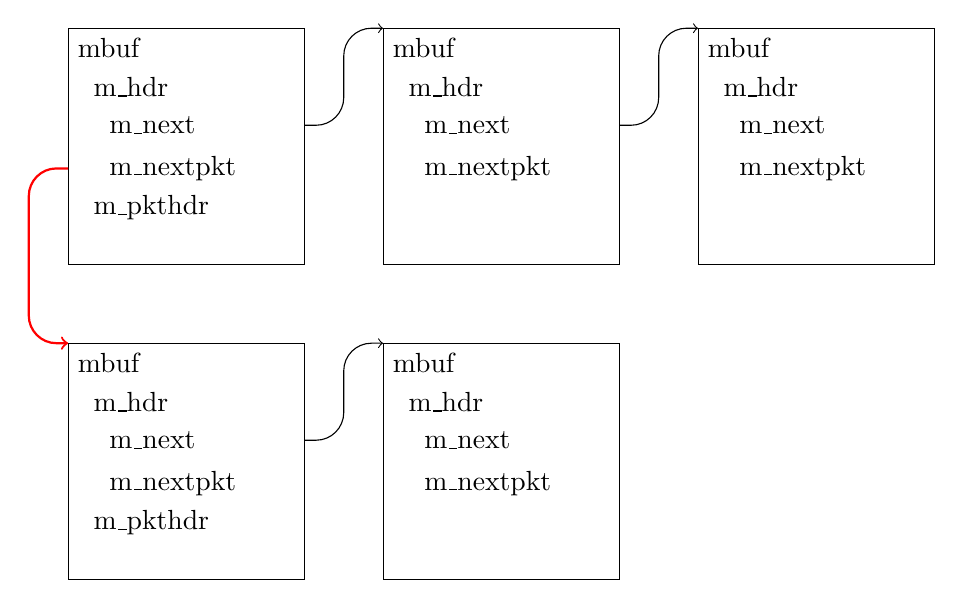
\begin{tikzpicture}
\draw
      ( 0  , 0  ) rectangle +(3,-3)
    ++( 0  , 0  ) node [below right] (mbuf00)     {mbuf}
    ++(  .2,- .5) node [below right]              {m\_hdr}
    ++(  .2,- .5) node [below right] (mnext00)    {m\_next}
    ++( 0  ,- .5) node [below right] (mnextpkt00) {m\_nextpkt}
    ++(- .2,- .5) node [below right]              {m\_pkthdr};
\draw
      ( 4  , 0  ) rectangle +(3,-3)
    ++( 0  , 0  ) node [below right] (mbuf01)     {mbuf}
    ++(  .2,- .5) node [below right]              {m\_hdr}
    ++(  .2,- .5) node [below right] (mnext01)    {m\_next}
    ++( 0  ,- .5) node [below right] (mnextpkt01) {m\_nextpkt};
\draw
      ( 8  , 0  ) rectangle +(3,-3)
    ++( 0  , 0  ) node [below right] (mbuf02)     {mbuf}
    ++(  .2,- .5) node [below right]              {m\_hdr}
    ++(  .2,- .5) node [below right] (mnext02)    {m\_next}
    ++( 0  ,- .5) node [below right] (mnextpkt02) {m\_nextpkt};
\draw[->,rounded corners=10]
    (mnext00 -| 3,0) -| (3.5,0) -- (4,0);
\draw[->,rounded corners=10]
    (mnext01 -| 7,0) -| (7.5,0) -- (8,0);

\draw
      ( 0  ,-4  ) rectangle +(3,-3)
    ++( 0  , 0  ) node [below right] (mbuf10)     {mbuf}
    ++(  .2,- .5) node [below right]              {m\_hdr}
    ++(  .2,- .5) node [below right] (mnext10)    {m\_next}
    ++( 0  ,- .5) node [below right] (mnextpkt10) {m\_nextpkt}
    ++(- .2,- .5) node [below right]              {m\_pkthdr};
\draw
      ( 4  ,-4  ) rectangle +(3,-3)
    ++( 0  , 0  ) node [below right] (mbuf11)     {mbuf}
    ++(  .2,- .5) node [below right]              {m\_hdr}
    ++(  .2,- .5) node [below right] (mnext11)    {m\_next}
    ++( 0  ,- .5) node [below right] (mnextpkt11) {m\_nextpkt};
\draw[->,rounded corners=10]
    (mnext10 -| 3,-4) -| (3.5,-4) -- (4,-4);
\draw[->,rounded corners=10,thick,red]
    (mnextpkt00 -| 0,0) -| (-.5,-4) -- (0,-4);
\end{tikzpicture}
\end{frame}

\begin{frame}{MBuf Cluster}
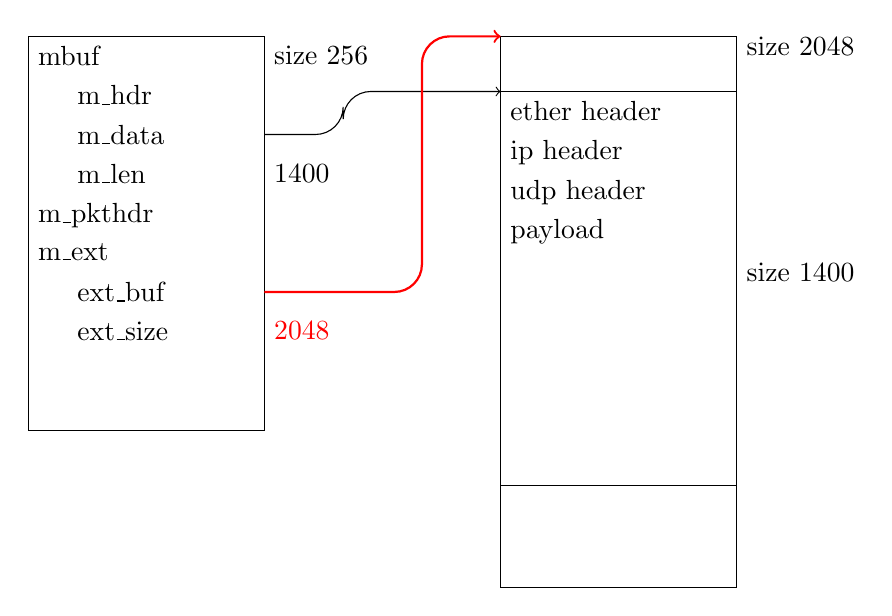
\begin{tikzpicture}
\draw
      ( 0  , 0  ) rectangle +(3,-5)
    ++( 0  , 0  ) node [below right] (mbuf)    {mbuf}
    ++(  .5,- .5) node [below right]           {m\_hdr}
    ++( 0  ,- .5) node [below right] (mdata)   {m\_data}
    ++( 0  ,- .5) node [below right] (mlen)    {m\_len}
    ++(- .5,- .5) node [below right]           {m\_pkthdr}
    ++( 0  ,- .5) node [below right]           {m\_ext}
    ++(  .5,- .5) node [below right] (extbuf)  {ext\_buf}
    ++( 0  ,- .5) node [below right] (extsize) {ext\_size};
\path
    (mbuf    -| 3,0) node [right] {size 256}
    (mlen    -| 3,0) node [right] {1400}
    (extsize -| 3,0) node [right,red] {2048};

\draw
      ( 6  , 0  ) rectangle +(3,-7)
    ++( 0  , 0  ) node [below right] (mcl)    {}
      ( 6  ,-.7 ) -- +(3,0)
    ++( 0  , 0  ) node [below right] {ether header}
    ++( 0  ,- .5) node [below right] {ip header}
    ++( 0  ,- .5) node [below right] {udp header}
    ++( 0  ,- .5) node [below right] {payload}
      ( 6  ,-5.7) -- +(3,0);
\path
    (mcl    -| 9,0) node [right] {size 2048}
      ( 9  ,  -3  ) node [right] {size 1400};
\draw[->,rounded corners=10]
    (mdata  -| 3,0) -| (4,-.7) -- (6,-.7);
\draw[->,rounded corners=10,thick,red]
    (extbuf -| 3,0) -| (5,0) -- (6,0);
\end{tikzpicture}
\end{frame}

\section{Packet Processing}

\begin{frame}{Packet Input}
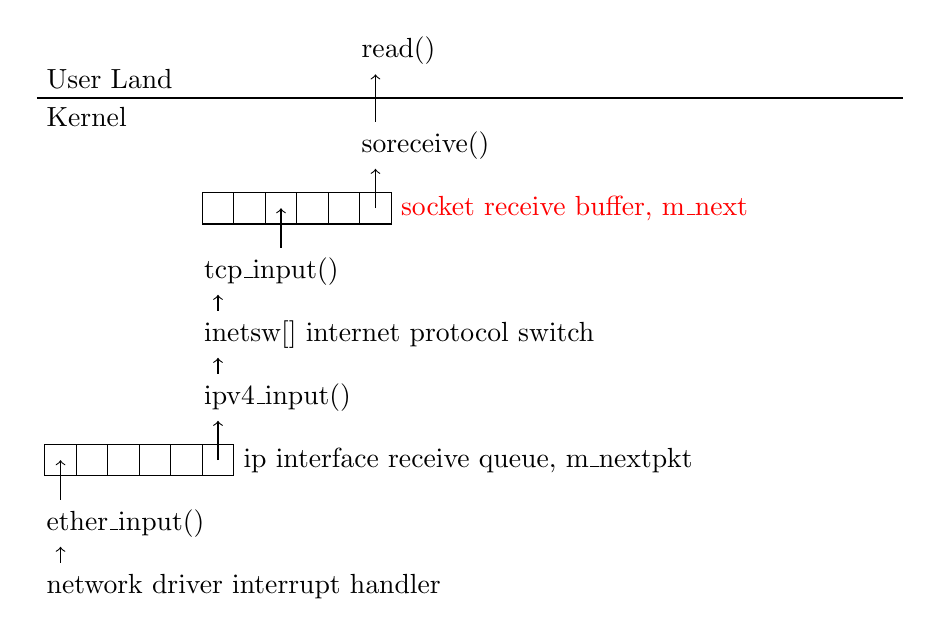
\begin{tikzpicture}
\draw (0,0)
    node (ni) [right] {network driver interrupt handler} ++(0,.8)
    node (ei) [right] {ether\_input()} ++(.1,.6)
    rectangle ++(.4,.4) rectangle ++(.4,-.4)
    rectangle ++(.4,.4) rectangle ++(.4,-.4)
    rectangle ++(.4,.4) rectangle ++(.4,-.4) ++(0,.2)
    node (rq) [right] {ip interface receive queue, m\_nextpkt} ++(-.5,.8)
    node (ii) [right] {ipv4\_input()} ++(0,.8)
    node (ps) [right] {inetsw[] internet protocol switch} ++(0,.8)
    node (ti) [right] {tcp\_input()} ++(.1,.6)
    rectangle ++(.4,.4) rectangle ++(.4,-.4)
    rectangle ++(.4,.4) rectangle ++(.4,-.4)
    rectangle ++(.4,.4) rectangle ++(.4,-.4) ++(0,.2)
    node (rb) [right,red] {socket receive buffer, m\_next} ++(-.5,.8)
    node (sr) [right] {soreceive()} ++(0,1.2)
    node (rd)  [right] {read()};
\draw[->] (node cs:name=ni,anchor=west) ++(.3,.3) -- ++(0,.2);
\draw[->] (node cs:name=ei,anchor=west) ++(.3,.3) -- ++(0,.5);
\draw[->] (node cs:name=rq,anchor=west) ++(-.2,0) -- ++(0,.5);
\draw[->] (node cs:name=ii,anchor=west) ++(.3,.3) -- ++(0,.2);
\draw[->] (node cs:name=ps,anchor=west) ++(.3,.3) -- ++(0,.2);
\draw[->] (node cs:name=ti,anchor=west) ++(1.1,.3) -- ++(0,.5);
\draw[->] (node cs:name=rb,anchor=west) ++(-.2,0) -- ++(0,.5);
\draw[->] (node cs:name=sr,anchor=west) ++(.3,.3) -- ++(0,.6);
\path (node cs:name=rd,anchor=west) ++(0,-.6) node (cs) {};
\draw[thick] (cs -| 0,0) node (context) {} -- +(11,0);
\node [below right] at (context) {Kernel};
\node [above right] at (context) {User Land};
\end{tikzpicture}
\end{frame}

\begin{frame}{Packet Output}
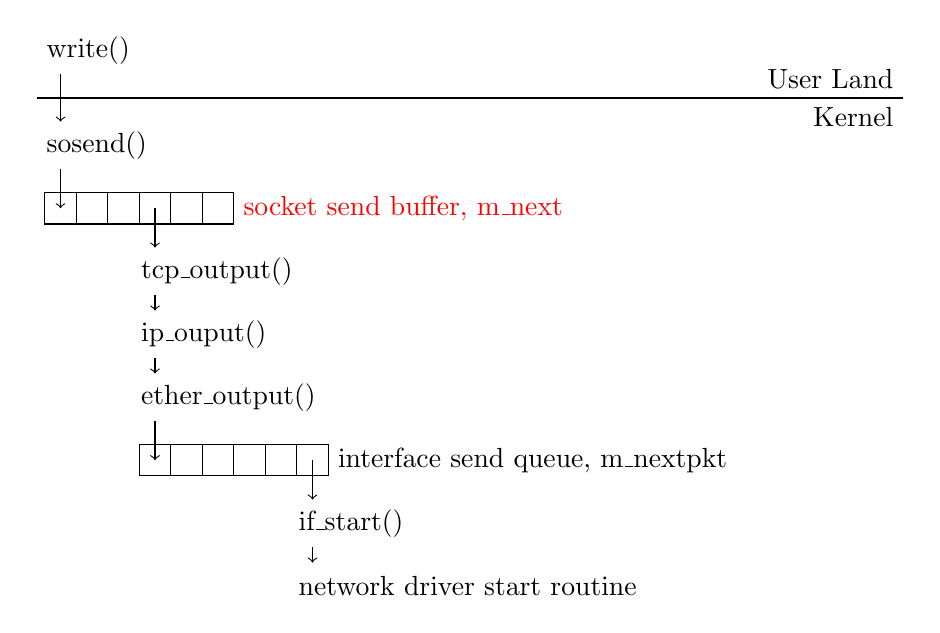
\begin{tikzpicture}
\draw (0,0)
    node (wr) [right] {write()} ++(0,-1.2)
    node (ss) [right] {sosend()} ++(.1,-.6)
    rectangle ++(.4,-.4) rectangle ++(.4,.4)
    rectangle ++(.4,-.4) rectangle ++(.4,.4)
    rectangle ++(.4,-.4) rectangle ++(.4,.4) ++(0,-.2)
    node (sb) [right,red] {socket send buffer, m\_next} ++(-1.3,-.8)
    node (to) [right] {tcp\_output()} ++(0,-.8)
    node (io) [right] {ip\_ouput()} ++(0,-.8)
    node (eo) [right] {ether\_output()} ++(.1,-.6)
    rectangle ++(.4,-.4) rectangle ++(.4,.4)
    rectangle ++(.4,-.4) rectangle ++(.4,.4)
    rectangle ++(.4,-.4) rectangle ++(.4,.4) ++(0,-.2)
    node (sq) [right] {interface send queue, m\_nextpkt} ++(-.5,-.8)
    node (is) [right] {if\_start()} ++(0,-.8)
    node (ns) [right] {network driver start routine};
\draw[->] (node cs:name=wr,anchor=west) ++(.3,-.3) -- ++(0,-.6);
\draw[->] (node cs:name=ss,anchor=west) ++(.3,-.3) -- ++(0,-.5);
\draw[->] (node cs:name=sb,anchor=west) ++(-1,0) -- ++(0,-.5);
\draw[->] (node cs:name=to,anchor=west) ++(.3,-.3) -- ++(0,-.2);
\draw[->] (node cs:name=io,anchor=west) ++(.3,-.3) -- ++(0,-.2);
\draw[->] (node cs:name=eo,anchor=west) ++(.3,-.3) -- ++(0,-.5);
\draw[->] (node cs:name=sq,anchor=west) ++(-.2,0) -- ++(0,-.5);
\draw[->] (node cs:name=is,anchor=west) ++(.3,-.3) -- ++(0,-.2);
\path (node cs:name=wr,anchor=west) ++(0,-.6) node (cs) {};
\draw[thick] (cs -| 0,0) -- +(11,0) node (context) {};
\node [below left] at (context) {Kernel};
\node [above left] at (context) {User Land};
\end{tikzpicture}
\end{frame}

\begin{frame}{Process Wakeup}
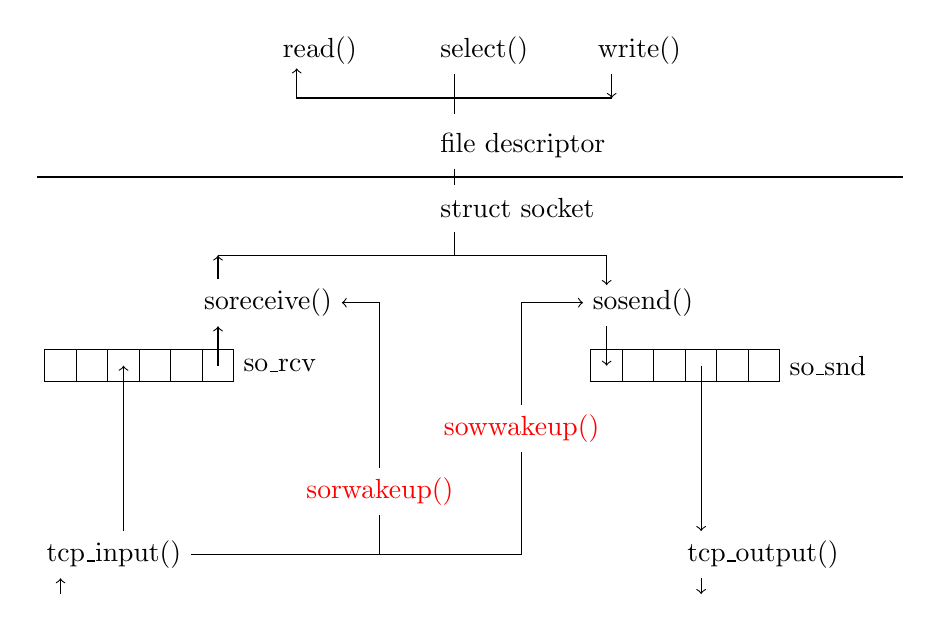
\begin{tikzpicture}
\draw (0,0)
    node (ti) [right] {tcp\_input()} ++(.1,2.2)
    rectangle ++(.4,.4) rectangle ++(.4,-.4)
    rectangle ++(.4,.4) rectangle ++(.4,-.4)
    rectangle ++(.4,.4) rectangle ++(.4,-.4) ++(0,.2)
    node (rb) [right] {so\_rcv} ++(-.5,.8)
    node (sr) [right] {soreceive()} ++(3,1.2)
    node (so) [right] {struct socket} ++(0,.8)
    node (fd) [right] {file descriptor} ++(-2,1.2)
    node (rd) [right] {read()} ++(2,0)
    node (sl) [right] {select()} ++(2,0)
    node (wr) [right] {write()};
\draw (sr) ++(4,0)
    node (ss) [right] {sosend()} ++(.1,-.6)
    rectangle ++(.4,-.4) rectangle ++(.4,.4)
    rectangle ++(.4,-.4) rectangle ++(.4,.4)
    rectangle ++(.4,-.4) rectangle ++(.4,.4) ++(0,-.2)
    node (sb) [right] {so\_snd} ++(-1.3,-2.4)
    node (to) [right] {tcp\_output()};
\draw[->]
    (node cs:name=ti,anchor=east) -| ++(2.4,.5) ++(0,.3)
    node (rw) [red] {sorwakeup()} ++(0,.3) |-
    (node cs:name=sr,anchor=east);
\draw[->]
    (node cs:name=ti,anchor=east) -| ++(4.2,1.3) ++(0,.3)
    node (rw) [red] {sowwakeup()} ++(0,.3) |-
    (node cs:name=ss,anchor=west);
\draw[->] (node cs:name=ti,anchor=west) ++(.3,-.5) -- ++(0,.2);
\draw[->] (node cs:name=ti,anchor=west) ++(1.1,.3) -- ++(0,2.1);
\draw[->] (node cs:name=rb,anchor=west) ++(-.2,0) -- ++(0,.5);
\draw[->] (node cs:name=sr,anchor=west) ++(.3,.3) -- ++(0,.3);
\path (node cs:name=ss,anchor=west) ++(.3,.1) node (ssn) {};
\draw[->] (node cs:name=sr,anchor=west) ++(.3,.6) -| (ssn);
\draw[->] (node cs:name=ss,anchor=west) ++(.3,-.3) -- ++(0,-.5);
\draw[->] (node cs:name=sb,anchor=west) ++(-1,0) -- ++(0,-2.1);
\draw[->] (node cs:name=to,anchor=west) ++(.3,-.3) -- ++(0,-.2);
\draw (node cs:name=sl,anchor=west) ++(.3,-.3) -- ++(0,-.5);
\draw (node cs:name=fd,anchor=west) ++(.3,-.3) -- ++(0,-.2);
\draw (node cs:name=so,anchor=west) ++(.3,-.3) -- ++(0,-.3);
\draw[->] (node cs:name=wr,anchor=west) ++(.3,-.3) -- ++(0,-.3);
\path (node cs:name=rd,anchor=west) ++(.3,-.1) node (rdn) {};
\draw[->] (node cs:name=wr,anchor=west) ++(.3,-.6) -| (rdn);
\path (node cs:name=fd,anchor=west) ++(0,-.4) node (cs) {};
\draw[thick] (cs -| 0,0) node (context) {} -- +(11,0);
\end{tikzpicture}
\end{frame}

\section{Socket Splicing}

\section{API}

\section{Application}

IPv4 IPv6
TCP UDP

\end{document}
